在下一节中，我们先引入 TT 矩阵，也称矩阵乘积算符（Matrix Product Operator, MPO），然后演示如何在 TT 格式下高效地完成各类运算。
\subsection{TT 格式下的高效运算}\label{sec:efficient-operations}
张量列（TT）格式的一个关键优势在于，它不仅给出高维张量的低秩表示，还使得关键代数运算能够高效执行。
本节给出可以在 TT 格式下高效执行的主要运算。我们先说明如何计算两个张量列（TT）张量之间的内积，接着引入大矩阵的矩阵乘积算符（MPO）表示，并讨论 TT 格式下的矩阵-向量乘积~(mat–vec)。然后讨论 TT 舍入，这是控制 TT 秩增长的关键步骤。最后概述 TT 框架中其他可高效执行的运算及其计算复杂度。
\paragraph{内积}
如第~\ref{subsec:contraction} 节所述，无论对张量还是对向量，内积都由连接所有对应指标得到。设 TT 格式下有两个四阶张量 $\Tt=\TT(({\Gt_n})_{n=1}^N)$、$\widetilde{\Tt}=\TT(({\Tilde{\Gt_n}})_{n=1}^N)\in\RR^{d_1\times...\times d_4}$，则该内积可以高效地算出，例如，
\begin{align}\label{eq:tt-inner}
\langle\Tt,\widetilde{\Tt}\rangle 
&=
    \begin{tikzpicture}[baseline=\baseline]
    \tikzset{tensor/.style = {minimum size = 0.5cm,shape = circle,thick,draw=black,inner sep = 0pt}, edge/.style   = {thick,line width=.4mm},every loop/.style={}}
    \def\y{0}
    \def\x{0}
  \node[tensor,fill=red!30!white] (G1) at (\x,\y+0.5){$\Gt_1$};
  \node[tensor,fill=red!50!white] (G2) at (\x+1,\y+0.5){$\Gt_2$};
  \node[tensor,fill=blue!50!white] (G3) at (\x+2,\y+0.5){$\Gt_3$};
   \node[tensor,fill=blue!20!white] (G4) at (\x+3,\y+0.5){$\Gt_4$};
\node[tensor,fill=red!30!white] (Gtilde1) at (\x,\y-0.5){$\Tilde{\Gt_1}$};
  \node[tensor,fill=red!50!white] (Gtilde2) at (\x+1,\y-0.5){$\Tilde{\Gt_2}$};
  \node[tensor,fill=blue!50!white] (Gtilde3) at (\x+2,\y-0.5){$\Tilde{\Gt_3}$};
   \node[tensor,fill=blue!20!white] (Gtilde4) at (\x+3,\y-0.5){$\Tilde{\Gt_4}$};
    \draw[edge](G1) -- (Gtilde1)node [midway,left] {\edgelabel{$d_1$}};
    \draw[edge](G2) -- (Gtilde2)node [midway,left] {\edgelabel{$d_2$}};
    \draw[edge](G3) -- (Gtilde3)node [midway,left] {\edgelabel{$d_4$}};
     \draw[edge](G4) -- (Gtilde4)node [midway,left] {\edgelabel{$d_1$}};
    \draw[edge](G1) -- (G2) node [midway,above] {\edgelabel{$R$}};
    \draw[edge](G2) -- (G3) node [midway,above] {\edgelabel{$R$}};
    \draw[edge](G3) -- (G4) node [midway,above] {\edgelabel{$R$}};
    \draw[edge](Gtilde1) -- (Gtilde2) node [midway,below] {\edgelabel{$R$}};
    \draw[edge](Gtilde2) -- (Gtilde3) node [midway,below] {\edgelabel{$R$}};
    \draw[edge](Gtilde3) -- (Gtilde4) node [midway,below] {\edgelabel{$R$}};
\end{tikzpicture}\nonumber\\
&=
\begin{tikzpicture}[baseline=\baseline]
    \tikzset{tensor/.style = {minimum size = 0.5cm,shape = circle,thick,draw=black,inner sep = 0pt}, edge/.style   = {thick,line width=.4mm},every loop/.style={}}
    \def\y{0}
    \def\x{0}
      \node[tensor,fill=red!30!white] (At_1) at (\x+4.2,\y){$\At_1$};
  \node[tensor,fill=red!50!white] (At_2) at (\x+5.5,\y){$\At_2$};
  \node[tensor,fill=blue!50!white] (At_3) at (\x+6.8,\y){$\At_3$};
   \node[tensor,fill=blue!20!white] (At_4) at (\x+8,\y){$\At_4$};
    \draw[edge](At_1) -- (At_2) node [midway,above] {\edgelabel{$R$}};
    \draw[edge](\x+4.45,\y-0.1) --  (\x+5.25,\y-0.1) node [midway,below] {\edgelabel{$R$}};
    \draw[edge](At_2) -- (At_3) node [midway,above] {\edgelabel{$R$}};
    \draw[edge](\x+5.75,\y-0.1) --  (\x+6.55,\y-0.1) node [midway,below] {\edgelabel{$R$}};
    \draw[edge](At_3) -- (At_4) node [midway,above] {\edgelabel{$R$}};
    \draw[edge](\x+7.05,\y-0.1) --  (\x+7.75,\y-0.1) node [midway,below] {\edgelabel{$R$}};
    \node[draw=none] at (\x+8.6,\y) {$=$};
    \node[tensor,fill=red!30!white] (At_1) at (\x+9.2,\y){$\At_1$};
  \node[tensor,fill=red!50!white] (At_2) at (\x+10.2,\y){$\At_2$};
  \node[tensor,fill=blue!50!white] (At_3) at (\x+11.2,\y){$\At_3$};
   \node[tensor,fill=blue!20!white] (At_4) at (\x+12.2,\y){$\At_4$};
    \draw[edge](At_1) -- (At_2) node [midway,above] {\edgelabel{$R^2$}};
    \draw[edge](At_2) -- (At_3) node [midway,above] {\edgelabel{$R^2$}};
    \draw[edge](At_3) -- (At_4) node [midway,above] {\edgelabel{$R^2$}};
    \end{tikzpicture},
\end{align}
其中，为简单起见，我们假设所有秩都等于 $R$。
按式~\eqref{eq:tt-inner} 所描述的过程计算 TT 格式下两个 $N$ 阶张量的内积，其复杂度为 $\bigo(NdR^4)$，这里假设 $d_1=\cdots=d_N=d$ 且 $R_1=\cdots=R_{N-1} = R$。与复杂度为 $\bigo(d^N)$ 的标准方法相比，这是一个显著的改进。因此，TT 格式为在高维且 TT 秩较低的张量上进行运算提供了高效而实用的途径。此外，核心张量还能以更高效的方式收缩：
\begin{align*}
\begin{tikzpicture}[baseline=\baseline]
    \tikzset{tensor/.style = {minimum size = 0.5cm,shape = circle,thick,draw=black,inner sep = 0pt}, edge/.style   = {thick,line width=.4mm},every loop/.style={}}
    \def\y{0}
    \def\x{0}
    \node[tensor,fill=red!30!white] (D) at (\x-1,\y){$\Gt_1$};
    \node[tensor,fill=red!50!white] (A) at (\x,\y){$\Gt_2$};
    \node[tensor,fill=blue!50!white] (B) at (\x+1,\y){$\Gt_3$};
    \node[tensor,fill=blue!20!white] (C) at (\x+2,\y){$\Gt_4$};
    \draw[edge](A) -- (\x,\y-0.7)node [midway,left] {\edgelabel{$d_2$}};
    \draw[edge](B) -- (\x+1,\y-0.7)node [midway,left] {\edgelabel{$d_3$}};
    \draw[edge](C) -- (\x+2,\y-0.7)node [midway,left] {\edgelabel{$d_4$}};
    \draw[edge](D) -- (\x-1,\y-0.7)node [midway,left] {\edgelabel{$d_1$}};
    \draw[edge](D) -- (A) node [midway,above] {\edgelabel{$R$}};
    \draw[edge](A) -- (B) node [midway,above] {\edgelabel{$R$}};
    \draw[edge](B) -- (C) node [midway,above] {\edgelabel{$R$}};
    \node[tensor,fill=red!30!white] (Dtild) at (\x-1,\y-1){$\Tilde{\Gt_1}$};
    \node[tensor,fill=red!50!white] (Atild) at (\x,\y-1){$\Tilde{\Gt_2}$};
    \node[tensor,fill=blue!50!white] (Btild) at (\x+1,\y-1){$\Tilde{\Gt_3}$};
    \node[tensor,fill=blue!20!white] (Ctild) at (\x+2,\y-1){$\Tilde{\Gt_4}$};
    \draw[edge](Dtild) -- (Atild) node [midway,below] {\edgelabel{$R$}};
    \draw[edge](Atild) -- (Btild) node [midway,below] {\edgelabel{$R$}};
    \draw[edge](Btild) -- (Ctild) node [midway,below] {\edgelabel{$R$}};
    \draw[thick, dotted,rotate=90] (\x-0.5,\y+1) ellipse (1 cm and 0.5 cm);
    \node[tensor,fill=red!30!white] (Gt_1) at (\x+3.5,\y){$\Gt_1$};
    \node[tensor,fill=red!50!white] (Gt_2) at (\x+4.5,\y){$\Gt_2$};
    \node[tensor,fill=blue!50!white] (Gt_3) at (\x+5.5,\y){$\Gt_3$};
    \node[tensor,fill=blue!20!white] (Gt_4) at (\x+6.5,\y){$\Gt_4$};
    \draw[edge](Gt_1) -- (Gt_2) node [midway,above]{\scalebox{0.7}{\dimcolor{$R$}}};
    \draw[edge](Gt_2) -- (Gt_3) node [midway,above,very near start]{\scalebox{0.7}{\dimcolor{$R$}}};
    \draw[edge](Gt_3) -- (Gt_4) node [midway,above]{\scalebox{0.7}{\dimcolor{$R$}}};
    \node[tensor,fill=red!30!white] (Gtild_1) at (\x+3.5,\y-1){$\Tilde{\Gt_1}$};
    \node[tensor,fill=red!50!white] (Gtild_2) at (\x+4.5,\y-1){$\Tilde{\Gt_2}$};
    \node[tensor,fill=blue!50!white] (Gtild_3) at (\x+5.5,\y-1){$\Tilde{\Gt_3}$};
    \node[tensor,fill=blue!20!white] (Gtild_4) at (\x+6.5,\y-1){$\Tilde{\Gt_4}$};
    \draw[edge](Gtild_1) -- (Gtild_2) node [midway,below,near end] {\scalebox{0.7}{\dimcolor{$R$}}};
    \draw[edge](Gtild_2) -- (Gtild_3) node [midway,below] {\scalebox{0.7}{\dimcolor{$R$}}};
    \draw[edge](Gtild_3) -- (Gtild_4) node [midway,below]{\scalebox{0.7}{\dimcolor{$R$}}};
    \draw[edge](Gt_1) -- (Gtild_1) node [midway,left] {\scalebox{0.7}{\dimcolor{$d_1$}}};
    \draw[edge](Gt_2) -- (Gtild_2) node [midway,left]{\scalebox{0.7}{\dimcolor{$d_2$}}};
    \draw[edge](Gt_3) -- (Gtild_3) node [midway,left]{\scalebox{0.7}{\dimcolor{$d_3$}}};
    \draw[edge](Gt_4) -- (Gtild_4) node [midway,left]{\scalebox{0.7}{\dimcolor{$d_4$}}};
    \node[draw=none] at (\x+2.6,\y-0.5){$\rightarrow$};
    \draw[dash pattern=on 1pt off 2pt] plot[smooth cycle] coordinates { 
    (\x+3,\y+0.35) 
    (\x+3.9, \y+0.35) (\x+4.9,\y+0.35) (\x+4.9, \y-0.35)  (\x+3.9,\y-0.35) (\x+3.9,\y-1.4) (\x+3, \y-1.4) };
    \node[tensor,fill=red!30!white] (Gt_1) at (\x+8,\y){$\Gt_1$};
    \node[tensor,fill=red!50!white] (Gt_2) at (\x+9,\y){$\Gt_2$};
    \node[tensor,fill=blue!50!white] (Gt_3) at (\x+10,\y){$\Gt_3$};
    \node[tensor,fill=blue!20!white] (Gt_4) at (\x+11,\y){$\Gt_4$};
    \draw[edge](Gt_1) -- (Gt_2) node [midway,above]{\scalebox{0.7}{\dimcolor{$R$}}};
    \draw[edge](Gt_2) -- (Gt_3) node [midway,above]{\scalebox{0.7}{\dimcolor{$R$}}};
    \draw[edge](Gt_3) -- (Gt_4) node [midway,above]{\scalebox{0.7}{\dimcolor{$R$}}};
    \node[tensor,fill=red!30!white] (Gtild_1) at (\x+8,\y-1){$\Tilde{\Gt_1}$};
    \node[tensor,fill=red!50!white] (Gtild_2) at (\x+9,\y-1){$\Tilde{\Gt_2}$};
    \node[tensor,fill=blue!50!white] (Gtild_3) at (\x+10,\y-1){$\Tilde{\Gt_3}$};
    \node[tensor,fill=blue!20!white] (Gtild_4) at (\x+11,\y-1){$\Tilde{\Gt_4}$};
    \draw[edge](Gtild_1) -- (Gtild_2) node [midway,below,] {\scalebox{0.7}{\dimcolor{$R$}}};
    \draw[edge](Gtild_2) -- (Gtild_3) node [midway,below] {\scalebox{0.7}{\dimcolor{$R$}}};
    \draw[edge](Gtild_3) -- (Gtild_4) node [midway,below]{\scalebox{0.7}{\dimcolor{$R$}}};
    \draw[edge](Gt_1) -- (Gtild_1) node [midway,left] {\scalebox{0.7}{\dimcolor{$d_1$}}};
    \draw[edge](Gt_2) -- (Gtild_2) node [midway,left]{\scalebox{0.7}{\dimcolor{$d_2$}}};
    \draw[edge](Gt_3) -- (Gtild_3) node [midway,left]{\scalebox{0.6}{\dimcolor{$d_3$}}};
    \draw[edge](Gt_4) -- (Gtild_4) node [midway,left]{\scalebox{0.7}{\dimcolor{$d_4$}}};
    \node[draw=none] at (\x+7.2,\y-0.5){$\rightarrow$};
    \draw[dash pattern=on 1pt off 2pt] plot[smooth cycle] coordinates { 
    (\x+7.7,\y+0.3) 
    (\x+9.25, \y+0.35) (\x+9.25,\y-1.4) (\x+7.6, \y-1.4)};
    \node[draw=none] at (\x+11.7,\y-0.5){$\rightarrow$};
\end{tikzpicture}
\end{align*}
\begin{align*}
    \begin{tikzpicture}[baseline=\baseline]
    \tikzset{tensor/.style = {minimum size = 0.5cm,shape = circle,thick,draw=black,inner sep = 0pt}, edge/.style   = {thick,line width=.4mm},every loop/.style={}}
    \def\y{0}
    \def\x{0}
    \node[tensor,fill=red!30!white] (Gt_1) at (\x,\y){$\Gt_1$};
    \node[tensor,fill=red!50!white] (Gt_2) at (\x+1,\y){$\Gt_2$};
    \node[tensor,fill=blue!50!white] (Gt_3) at (\x+2,\y){$\Gt_3$};
    \node[tensor,fill=blue!20!white] (Gt_4) at (\x+3,\y){$\Gt_4$};
    \node[tensor,fill=red!30!white] (Gtild_1) at (\x,\y-1){$\Tilde{\Gt_1}$};
    \node[tensor,fill=red!50!white] (Gtild_2) at (\x+1,\y-1){$\Tilde{\Gt_2}$};
    \node[tensor,fill=blue!50!white] (Gtild_3) at (\x+2,\y-1){$\Tilde{\Gt_3}$};
    \node[tensor,fill=blue!20!white] (Gtild_4) at (\x+3,\y-1){$\Tilde{\Gt_4}$};
    \draw[edge](Gt_1) -- (Gtild_1)node [midway,left] {\edgelabel{$d_1$}};
    \draw[edge](Gt_2) -- (Gtild_2)node [midway,left] {\edgelabel{$d_2$}};
    \draw[edge](Gt_3) -- (Gtild_3)node [midway,left] {\edgelabel{$d_3$}};
    \draw[edge](Gt_4) -- (Gtild_4)node [midway,left] {\edgelabel{$d_4$}};
    \draw[edge](Gt_1) -- (Gt_2) node [midway,above] {\edgelabel{$R$}};
    \draw[edge](Gt_2) -- (Gt_3) node [midway,above] {\edgelabel{$R$}};
    \draw[edge](Gt_3) -- (Gt_4) node [midway,above,near end] {\scalebox{0.7}{\dimcolor{$R$}}};
    \draw[edge](Gtild_1) -- (Gtild_2) node [midway,below,near end] {\scalebox{0.7}{\dimcolor{$R$}}};
    \draw[edge](Gtild_2) -- (Gtild_3) node [midway,below] {\edgelabel{$R$}};
    \draw[edge](Gtild_3) -- (Gtild_4) node [midway,below] {\edgelabel{$R$}};
    \draw[dash pattern=on 1pt off 2pt] plot[smooth cycle] coordinates { 
    (\x-0.5,\y+0.5) (\x,\y+0.5)
    (\x+2.3, \y+0.5) (\x+2.3,\y-0.4) (\x+0.5, \y-0.4)  (\x+0.5, \y-1.34) (\x-0.5, \y-1.34) (\x-0.5, \y+0.1)};
    \node[draw=none] at (\x+3.7,\y-0.5){$\rightarrow$};
    \node[draw=none] at (\x+4.5,\y-0.5){$\cdots$};
    \node[draw=none] at (\x+5.5,\y-0.5){$\rightarrow$};
\end{tikzpicture}
\begin{tikzpicture}[baseline=\baseline]
    \tikzset{tensor/.style = {minimum size = 0.5cm,shape = circle,thick,draw=black,inner sep = 0pt}, edge/.style   = {thick,line width=.4mm},every loop/.style={}}
    \def\y{0}
    \def\x{0}
    \node[tensor,fill=red!30!white] (Gt_1) at (\x+6,\y){$\Gt_1$};
    \node[tensor,fill=red!50!white] (Gt_2) at (\x+7,\y){$\Gt_2$};
    \node[tensor,fill=blue!50!white] (Gt_3) at (\x+8,\y){$\Gt_3$};
    \node[tensor,fill=blue!20!white] (Gt_4) at (\x+9,\y){$\Gt_4$};
    \node[tensor,fill=red!30!white] (Gtild_1) at (\x+6,\y-1){$\Tilde{\Gt_1}$};
    \node[tensor,fill=red!50!white] (Gtild_2) at (\x+7,\y-1){$\Tilde{\Gt_2}$};
    \node[tensor,fill=blue!50!white] (Gtild_3) at (\x+8,\y-1){$\Tilde{\Gt_3}$};
    \node[tensor,fill=blue!20!white] (Gtild_4) at (\x+9,\y-1){$\Tilde{\Gt_4}$};
    \draw[edge](Gt_1) -- (Gtild_1)node [midway,left] {\edgelabel{$d_1$}};
    \draw[edge](Gt_2) -- (Gtild_2)node [midway,left] {\edgelabel{$d_2$}};
    \draw[edge](Gt_3) -- (Gtild_3)node [midway,left] {\edgelabel{$d_3$}};
    \draw[edge](Gt_4) -- (Gtild_4)node [midway,left] {\edgelabel{$d_4$}};
    \draw[edge](Gt_1) -- (Gt_2) node [midway,above] {\edgelabel{$R$}};
    \draw[edge](Gt_2) -- (Gt_3) node [midway,above] {\edgelabel{$R$}};
    \draw[edge](Gt_3) -- (Gt_4) node [midway,above] {\scalebox{0.65}{\textcolor{gray}{$R$}}};
    \draw[edge](Gtild_1) -- (Gtild_2) node [midway,below] {\scalebox{0.65}{\textcolor{gray}{$R$}}};
    \draw[edge](Gtild_2) -- (Gtild_3) node [midway,below] {\edgelabel{$R$}};
    \draw[edge](Gtild_3) -- (Gtild_4) node [midway,below,near end] {\edgelabel{$R$}};
    \draw[dash pattern=on 1pt off 2pt] plot[smooth cycle] coordinates { 
    (\x+5.5,\y+0.5) (\x+6,\y+0.5)
    (\x+9.5, \y+0.5) (\x+9.5,\y-0.4) (\x+8.3, \y-0.4)  (\x+8.3, \y-1.34) (\x+5.5, \y-1.34) (\x+5.5, \y+0.1)};
\end{tikzpicture}
\end{align*}
由上可见，计算两个长度为 $\bigo(d^N)$ 的向量的内积，其复杂度可降至 $\bigo(NdR^3)$。一般而言，为任意张量网络确定最优收缩顺序是一个 NP 难问题~\citep{chi1997optimizing}。
\paragraph{矩阵乘积算符~(MPO)}\label{par:mpo}
作为 TT 分解的推广，我们引入矩阵乘积算符（MPO）~\citep{oseledets2010approximation}。MPO 又称 TT 矩阵，是一条由四阶张量组成的链，用来表示一个矩阵。它最初是为描述作用于多体量子系统的算符而发展起来的。简单地说，MPO 就是一种用张量表示矩阵的方法。设有矩阵 $\Ab\in\RR^{I_1I_2\dots I_N\times J_1J_2\dots J_N}$。对 $n\in[N]$，令  $\At_n\in\RR^{R_{n-1}\times I_n\times J_n\times R_n}$ ，其中 $R_0=R_N=1$。$\Ab$ 的秩为 $(R_1,\cdots,R_N)$ 的 MPO 分解定义为 
$$\Ab_{i_1i_2\dotsi_N,j_1j_2\dots j_N} = (\At_1)_{i_1,j_1,:}(\At_2)_{:,i_2,j_2,:}\dots(\At_{N-1})_{:,i_{N-1},j_{N-1},:}(\At_N)_{:,i_N,j_N},$$ 
对所有指标 $i_1\in[I_1],\cdots,i_N\in[I_N]$ 与 $j_1\in[J_1],\dots, j_N\in[J_N]$ 成立。
下面用张量网络记法给出矩阵 $\Ab\in\RR^{I_1I_2I_3\times J_1J_2J_3}$ 的一个秩~$(R_1,R_2)$ MPO 分解的例子：
$$
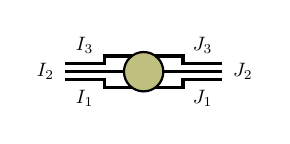
\begin{tikzpicture}[baseline=-0.5ex]
    \tikzset{tensor/.style = {minimum size = 0.5cm,shape = circle,thick,draw=black,inner sep = 0pt}, edge/.style = {thick,line width=.4mm},every loop/.style={}}
    \def\x{6}
    \def\y{0}
     \node[tensor,fill=green!50!red!50!white] (B) at (\x+1,\y) {$\Ab$};
    \draw[edge] (\x+1.15,\y+0.2) -- (\x+1.5,\y+0.2) -- (\x+1.5,\y+0.1) -- (\x+2,\y+0.1) node [midway,above]
    {\scalebox{0.7}{\dimcolor{$J_3$}}};
     \draw[edge] (B) -- (\x+2,\y)node [right]
    {\scalebox{0.7}{\dimcolor{$J_2$}}};
    \draw[edge] (\x+1.15,\y-0.2) -- (\x+1.5,\y-0.2)-- (\x+1.5,\y-0.1)-- (\x+2,\y-0.1) node [midway,below]
    {\scalebox{0.7}{\dimcolor{$J_1$}}};
    
     \draw[edge] (\x+0.85,\y+0.2) -- (\x+0.5,\y+0.2) -- (\x+0.5,\y+0.1) -- (\x,\y+0.1) node [midway,above]
    {\scalebox{0.7}{\dimcolor{$I_3$}}};
     \draw[edge] (B) -- (\x,\y)node [left]
    {\scalebox{0.7}{\dimcolor{$I_2$}}};

    \draw[edge] (\x+0.85,\y-0.2) -- (\x+0.5,\y-0.2)-- (\x+0.5,\y-0.1)-- (\x,\y-0.1) node [midway,below]
    {\scalebox{0.7}{\dimcolor{$I_1$}}};
\end{tikzpicture}
=
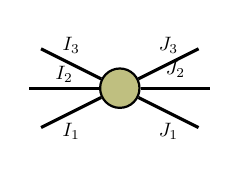
\begin{tikzpicture}[baseline=-0.5ex]
    \tikzset{tensor/.style = {minimum size = 0.5cm,shape = circle,thick,draw=black,inner sep = 0pt}, edge/.style = {thick,line width=.4mm},every loop/.style={}}
    \def\x{6}
    \def\y{0}
     \node[tensor,fill=green!50!red!50!white] (B) at (\x+1,\y) {$\At$};
    \draw[edge] (B) -- (\x-0.15,\y) node [midway,above=-0.07cm] {\scalebox{0.7}{\dimcolor{$I_2$}}};
    \draw[edge] (B) -- (\x,\y-0.5) node [midway,below] {\scalebox{0.7}{\dimcolor{$I_1$}}};
    \draw[edge] (B) -- (\x,\y+0.5) node [midway,above] {\scalebox{0.7}{\dimcolor{$I_3$}}};
    \draw[edge] (B) -- (\x+2.15,\y) node [midway,above=-0.07] {\scalebox{0.7}{\dimcolor{$J_2$}}};
    \draw[edge] (B) -- (\x+2,\y-0.5) node [midway,below] {\scalebox{0.7}{\dimcolor{$J_1$}}};
    \draw[edge] (B) -- (\x+2,\y+0.5) node [midway,above] {\scalebox{0.7}{\dimcolor{$J_3$}}};
\end{tikzpicture}
=
\begin{tikzpicture}[baseline=\baseline]
    \tikzset{tensor/.style = {minimum size = 0.5cm,shape = circle,thick,draw=black,inner sep = 0pt}, edge/.style   = {thick,line width=.4mm},every loop/.style={}}
    \def\y{0}
    \def\x{0}
  \node[tensor,fill=red!30!white] (D) at (\x-1.5,\y){$\At_1$};
  \node[tensor,fill=red!50!white] (A) at (\x,\y){$\At_2$};
  \node[tensor,fill=blue!50!white] (B) at (\x+1.5,\y){$\At_3$};
    \draw[edge](A) -- (\x,\y-0.75)node [midway, right] {\edgelabel{$I_2$}};
    \draw[edge](B) -- (\x+1.5,\y-0.75)node [midway,right] {\edgelabel{$I_3$}};
     \draw[edge](D) -- (\x-1.5,\y-0.75)node [midway,right] {\edgelabel{$I_1$}};
    \draw[edge](D) -- (A) node [midway,above] {\edgelabel{$R_1$}};
    \draw[edge](A) -- (B) node [midway,above] {\edgelabel{$R_2$}};
    \draw[edge](A) -- (\x,\y+0.75)node [midway, right] {\edgelabel{$J_2$}};
    \draw[edge](B) -- (\x+1.5,\y+0.75) node [midway,right] {\edgelabel{$J_3$}};
    \draw[edge](D) -- (\x-1.5,\y+0.75)node [midway,right] {\edgelabel{$J_1$}};
\end{tikzpicture}
=
\begin{tikzpicture}[baseline=\baseline]
    \tikzset{tensor/.style = {minimum size = 0.5cm,shape = circle,thick,draw=black,inner sep = 0pt}, edge/.style   = {thick,line width=.4mm},every loop/.style={}}
    \def\y{0}
    \def\x{0}
  \node[tensor,fill=red!30!white] (D) at (\x-1.5,\y){$\At_1$};
  \node[tensor,fill=red!50!white] (A) at (\x,\y){$\At_2$};
  \node[tensor,fill=blue!50!white] (B) at (\x+1.5,\y){$\At_3$};
    \draw[edge](A) -- (\x,\y-1.25)node [near start=-0.05, right=-0.07cm] {\edgelabel{$I_2$}};
    \draw[edge](B) -- (\x+1.5,\y-0.75)-- (\x+0.15,\y-0.75)node [midway,below] {\edgelabel{$I_3$}}--(\x+0.15,\y-1.25);
     \draw[edge](D) -- (\x-1.5,\y-0.75)-- (\x-0.15,\y-0.75)node [midway,below] {\edgelabel{$I_1$}}--(\x-0.15,\y-1.25);
    \draw[edge](D) -- (A) node [midway,above] {\edgelabel{$R_1$}};
    \draw[edge](A) -- (B) node [midway,above] {\edgelabel{$R_2$}};
    \draw[edge](A) -- (\x,\y+1.25)node [near start=-0.05, right=-0.07cm] {\edgelabel{$J_2$}};
    \draw[edge](B) -- (\x+1.5,\y+0.75)-- (\x+0.15,\y+0.75)node [midway,above] {\edgelabel{$J_3$}}--(\x+0.15,\y+1.25);
    \draw[edge](D) -- (\x-1.5,\y+0.75)-- (\x-0.15,\y+0.75)node [midway,above] {\edgelabel{$J_1$}}--(\x-0.15,\y+1.25);
\end{tikzpicture}.
$$
\paragraph{MPO 中的矩阵-向量乘积} 矩阵 

